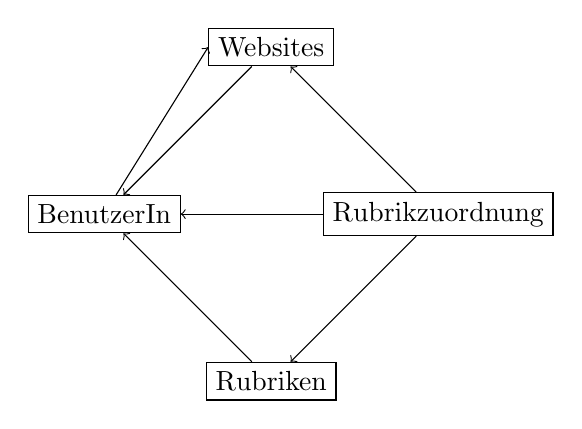
\begin{tikzpicture}[->, node distance=3cm]
\node[draw] (Websites) at (0,0) {Websites};
\node[draw] (BenutzerIn) [below left of= Websites] {BenutzerIn};
\node[draw] (Rubrikzuordnung) [below right of= Websites] {Rubrikzuordnung};
\node[draw] (Rubriken) [below right of= BenutzerIn] {Rubriken};

\draw[->] (Websites) 		-- (BenutzerIn);
\draw[->] (Rubrikzuordnung) -- (BenutzerIn);
\draw[->] (Rubriken) 		-- (BenutzerIn);
\draw[->] (BenutzerIn) 		-- (Websites.west);
\draw[->] (Rubrikzuordnung) -- (Websites);
\draw[->] (Rubrikzuordnung) -- (Rubriken);


\end{tikzpicture}